\smalltitle{سوال 3}\\
در ابتدا به شکل زیر توجه کنید:
\begin{figure}[H]
    \centerline{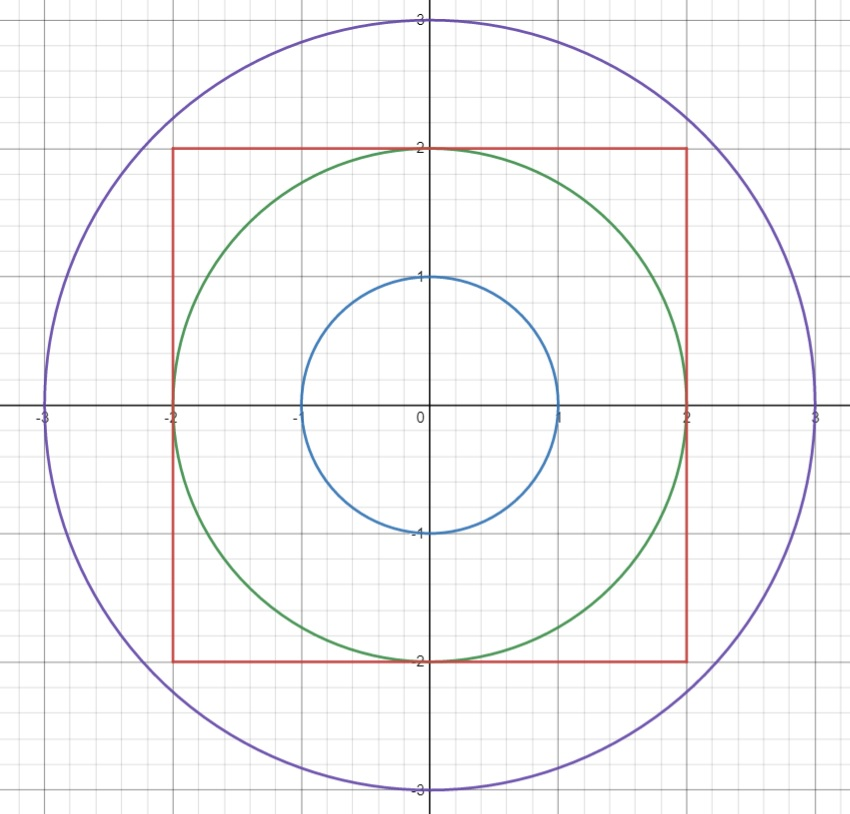
\includegraphics[scale=0.35]{pics/3.jpg}}
\end{figure}
در ابتدا باید ببینیم که چند درصد مساحت بین دایره‌ی بنفش و سبز، مربع قرمز رنگ است.
مساحت فاصله‌ی دو دایره به صورت
$(3r_0)^2 \pi - (2r_0)^2 \pi = 5r_0^2 \pi$
است. حال مساحت مربع را از دایره‌ی سبز کم می‌کنیم که مساحت مربع در دایره‌ی بنفش را بدست بیاوریم:
$(4r_0)^2 - (2r_0)^2 \pi = 4 r_0^2 (4 - \pi)$
پس نسبت مساحت مربع به دایره (مساحتی که فقط در پوسته‌ی بین دایره‌ی سبز و بنفش است)
برابر است با
$\frac{4 r_0^2 (4 - \pi)}{5r_0^2 \pi} = \frac{16 - 4\pi}{5 \pi} \approx 0.22$

حال به محاسبه‌ی احتمال برخورد تیر به داخلی‌ترین دایره را حساب می‌کنیم.
\begin{gather*}
p + \frac{p}{2} + \frac{p}{4} + \cdots = 1 = p (\underbrace{1 + \frac{1}{2} + \frac{1}{4} + \cdots}_{2})
\implies p = \frac{1}{2}
\end{gather*}
حال احتمال خوردن تیر به مساحت داخل مربع ولی خارج دایره‌ی سبز را حساب می‌کنیم:
$\frac{1}{8} \times 0.22 = 0.0275$
در نهایت احتمال‌ها را با هم جمع می‌کنیم:
\begin{gather*}
    \frac{1}{2} + \frac{1}{4} + 0.0275 = 0.7775
\end{gather*}